
\section{Galactic Chemical Evolution Models}
\label{outflows:sec:gce}
We now construct GCE models to understand the origin of the radial age and
metallicity gradients characterized in~\S~\ref{outflows:sec:empirical}.
To this end, we construct models describing the Galaxy disk as a series of
one-zone models like those in Chapters~\ref{bursts} and~\ref{dga} and
multi-ring models like those in Chapters~\ref{migration} and~\ref{ohno}.
Though similar, the former does not incorporate mixing of stellar populations
while the latter does.
We also extend these models to incorporate radial gas
flows~\citep[e.g.,][]{Lacey1985, Bilitewski2012}.
We present models with both analytic and numerical solutions.


\subsection{One-Zone Models}
\label{outflows:sec:gce:onezone}
The fundamental assumption of one-zone GCE models is instantaneous
mixing of newly produced metals in the star-forming ISM.
In the presence of accretion, star formation, and outflows, the rate of
change of the ISM gas mass~$M_g$ can be expressed as
\begin{equation}\begin{split}
\dot{M}_g &= \dot{M}_\text{in} - \dot{M}_\star - \dot{M}_\text{out} +
\dot{M}_r
\\
&\approx \dot{M}_\text{in} - \dot{M}_\star(1 + \eta - r),
\label{outflows:eq:mdot-gas}
\end{split}\end{equation}
where~$\dot{M}_r$ is the rate of recycling from stellar envelopes being
returned back to the ISM.
Though this rate in detail depends on the initial mass function
\citep[IMF; e.g.,][]{Salpeter1955, Kroupa2001, Chabrier2003}, the
initial-final remnant mass relation~\citep[e.g.,][]{Kalirai2008}, and the
mass-lifetime relation~\citep[e.g.,][]{Larson1974, Maeder1989, Hurley2000},
to first order it is quite fast for young stellar populations but then
slows considerably due to the long lifetimes of low-mass stars.
As a result, it is sufficiently accurate for the purposes of analytic
approximations to take a constant value~$r$ that is returned immediately
after a stellar population forms ($r \approx +0.4$ for
a~\citealt{Kroupa2001} IMF; see discussion in~\citealt{Weinberg2017b}).
\par
We have also substituted the ``mass-loading factor''
$\eta \equiv \dot{M}_\text{out} / \dot{M}_\star$ into the above expression,
which is of central interest to this chapter.
This parameter describes how much ambient ISM is swept up and lost to outflows
due to feedback.
As discussed in~\S~\ref{outflows:sec:intro}, GCE models of the Milky Way
tend to fall into one of two categories: those with~$\eta = 0$ everywhere
\citep[e.g.,][]{Spitoni2021}, and those in which it grows exponentially
with radius~\citep[e.g.,][]{Johnson2021}.
\par
In the present chapter, we focus on the abundances of alpha and
iron-peak elements whose production is dominated by SNe
\citep[e.g.,][]{Johnson2019}.
We take O and Fe as the prototypical elements from these categories, though
we would expect our GCE models to make similar predictions if we chose
differently.
The rate of change of the mass of some element~$x$ in the ISM can be
expressed as
\begin{equation}
\dot{M}_x = \ycc{$x$} \dot{M}_\star +
\yia{$x$} \langle \dot{M}_\star \rangle_\text{Ia} -
Z_x \dot{M}_\star \left(1 + \eta - r\right),
\label{outflows:eq:mdot-element}
\end{equation}
where~$Z_x$ is the abundance by mass of~$x$ in the ISM at a given moment in
time and~\ycc{$x$} and~\yia{$x$} are the population-averaged yields of~$x$
from core collapse supernovae (CCSNe) and Type Ia supernovae (SNe Ia),
respectively.
This parameterization assumes that all CCSNe yields are ejected immediately
following a stellar population's formation, which is valid as long as the
timescales of Galaxy evolution are significantly longer than the lifetimes
of massive stars.
Enrichment by SNe Ia is instead weighted by a delay-time distribution (DTD),
for which we retain the~$t^{-1.1}$ formalism from previous chapters as
suggested by comparisons of the cosmic SFH~\citep[e.g.,][]{Madau2017,
Driver2018} with volumetric SN Ia rates as a function of
redshift~\citep{Maoz2012a, Maoz2012b, Graur2013, Graur2014}.
\par
\citet{Weinberg2017b} demonstrate that the first-order details of the
enrichment history of alpha and iron-peak elements are established by
the mass-loading factor~$\eta$ and the star formation efficiency (SFE)
timescale~$\tau_\star \equiv M_g / \dot{M}_\star$ relating the
gas supply and the star formation rate (SFR).
The SFE timescale sets the position of the ``knee'' in the~\afe-\feh~plane,
while~$\eta$ controls the equilibrium abundance at which enrichment is
balanced by losses to outflows, which sets the end-point of the track.
The detailed form of the SFH has little impact, instead influencing how
stars distribute themselves along the track.
However, the detailed SFH has much more impact on the abundance evolution
in the~$\eta = 0$ scenario.
In this case, radial gas flows~\citep[e.g.,][]{Lacey1985}
also have a much stronger effect since the substantial sink term of
outflows is removed.
\par
To this end, we construct a parameterization for including the effects of
radial gas flows in one-zone GCE models.
Though the gas in any given region of the Galaxy should have a distribution of
velocities, the bulk flow is generally directed inward (i.e.,~$v_R < 0$).
The angular momentum of the disk gas is diluted by ongoing accretion, causing
material to subsequently fall toward the Galactic center~\citep{Bilitewski2012}.
In Appendix~\ref{outflows:sec:coefficients-derivation}, we consider a gas disk
whose surface density declines exponentially with radius and whose abundance
gradient has reached some steady-state equilibrium as suggested by our
empirical measurements in section~\ref{outflows:sec:empirical}.
Under the approximation that all of the gas is moving inward with the same
velocity~$v_R$, we demonstrate that the impact of radial flows on enrichment
rates and the gas supply can be expressed as
\begin{subequations}\begin{align}
\begin{split}
\dot{M}_{g,\flow} &= \dot{M}_\star \gamma_\flow
\\
\implies \dot{M}_g &= \dot{M}_\text{in} - \dot{M}_\star
\left(1 + \eta - \gamma_\flow - r\right)
\label{outflows:eq:mdot-gas-flow}
\end{split}
\\
\begin{split}
\dot{M}_{x,\flow} &= Z_x \dot{M}_\star \mu_\flow
\\
\implies \dot{M}_x &= \ycc{$x$} \dot{M}_\star +
\yia{$x$} \langle \dot{M}_\star \rangle_\text{Ia} -
Z_x \dot{M}_\star \left(1 + \eta - \mu_\flow - r\right).
\label{outflows:eq:mdot-element-flow}
\end{split}
\end{align}\end{subequations}
The flow coefficients~$\gamma_\flow$ and~$\mu_\flow$ are given by
\begin{subequations}\begin{align}
\gamma_\flow &\equiv -\tau_\star v_R
\left(\frac{1}{R} - \frac{1}{R_g}\right)
\label{outflows:eq:gamma-flow}
\\
\mu_\flow &\equiv -\tau_\star v_R
\left(\frac{1}{R} - \frac{1}{R_g} - \frac{1}{R_x}\right),
\label{outflows:eq:mu-flow}
\end{align}\end{subequations}
where~$R$ denotes Galactocentric radius,~$R_g$ is the scale radius of the gas
disk, and~$R_x \equiv -(\grad{X}~\ln 10)^{-1}$ is the scale radius of the
exponential metallicity gradient~$Z_x \propto e^{-R / R_x}$ implied by a linear
gradient in [X/H].
\par
We reserve the detailed derivation of~$\gamma_\flow$ and~$\mu_\flow$ for
Appendix~\ref{outflows:sec:coefficients-derivation} and provide only
qualitative justification of their functional forms here.
First and foremost, the linear dependence on~$v_R$ is expected -- as the flow
velocity increases, its effect on enrichment rates and the gas supply increases
proportionally (we remind the reader that~$v_R < 0 \implies -v_R > 0$ for an
inward flow).
The linear dependence on~$\tau_\star$ arises because these rates are tied to
the local gas supply.
When multiplied by the SFR in equations~\refp{outflows:eq:mdot-gas-flow}
and~\refp{outflows:eq:mdot-element-flow},~$\dot{M}_\star \tau_\star$ becomes
$M_g$ by definition.
The term~$-1 / R_g$ encodes the decrease in the surface density of gas with
increasing~$R$.
For centrally concentrated surface density gradients (i.e., small~$R_g$),
the flow coefficients decrease relative to their counterparts in more extended
disks as there is less gas at a slightly larger radius of~$R + \Delta R$.
An additional~$-1 / R_x$ term appears in the expression for~$\mu_\flow$ for
similar reasons -- the metal abundance is also lower at~$R + \Delta R$ due to
the radial gradient.
Lastly, both coefficients have a~$+1 / R$ term that arises due to the change in
area of an annulus~$2 \pi R \Delta R$ with radius.
This term encodes the ``pile-up'' of both gas and metals at small radii due to
the inward flow.
\par
{\color{red} Brief description of how~$\tau_\star$ should change with radius.}

\begin{figure*}
\centering
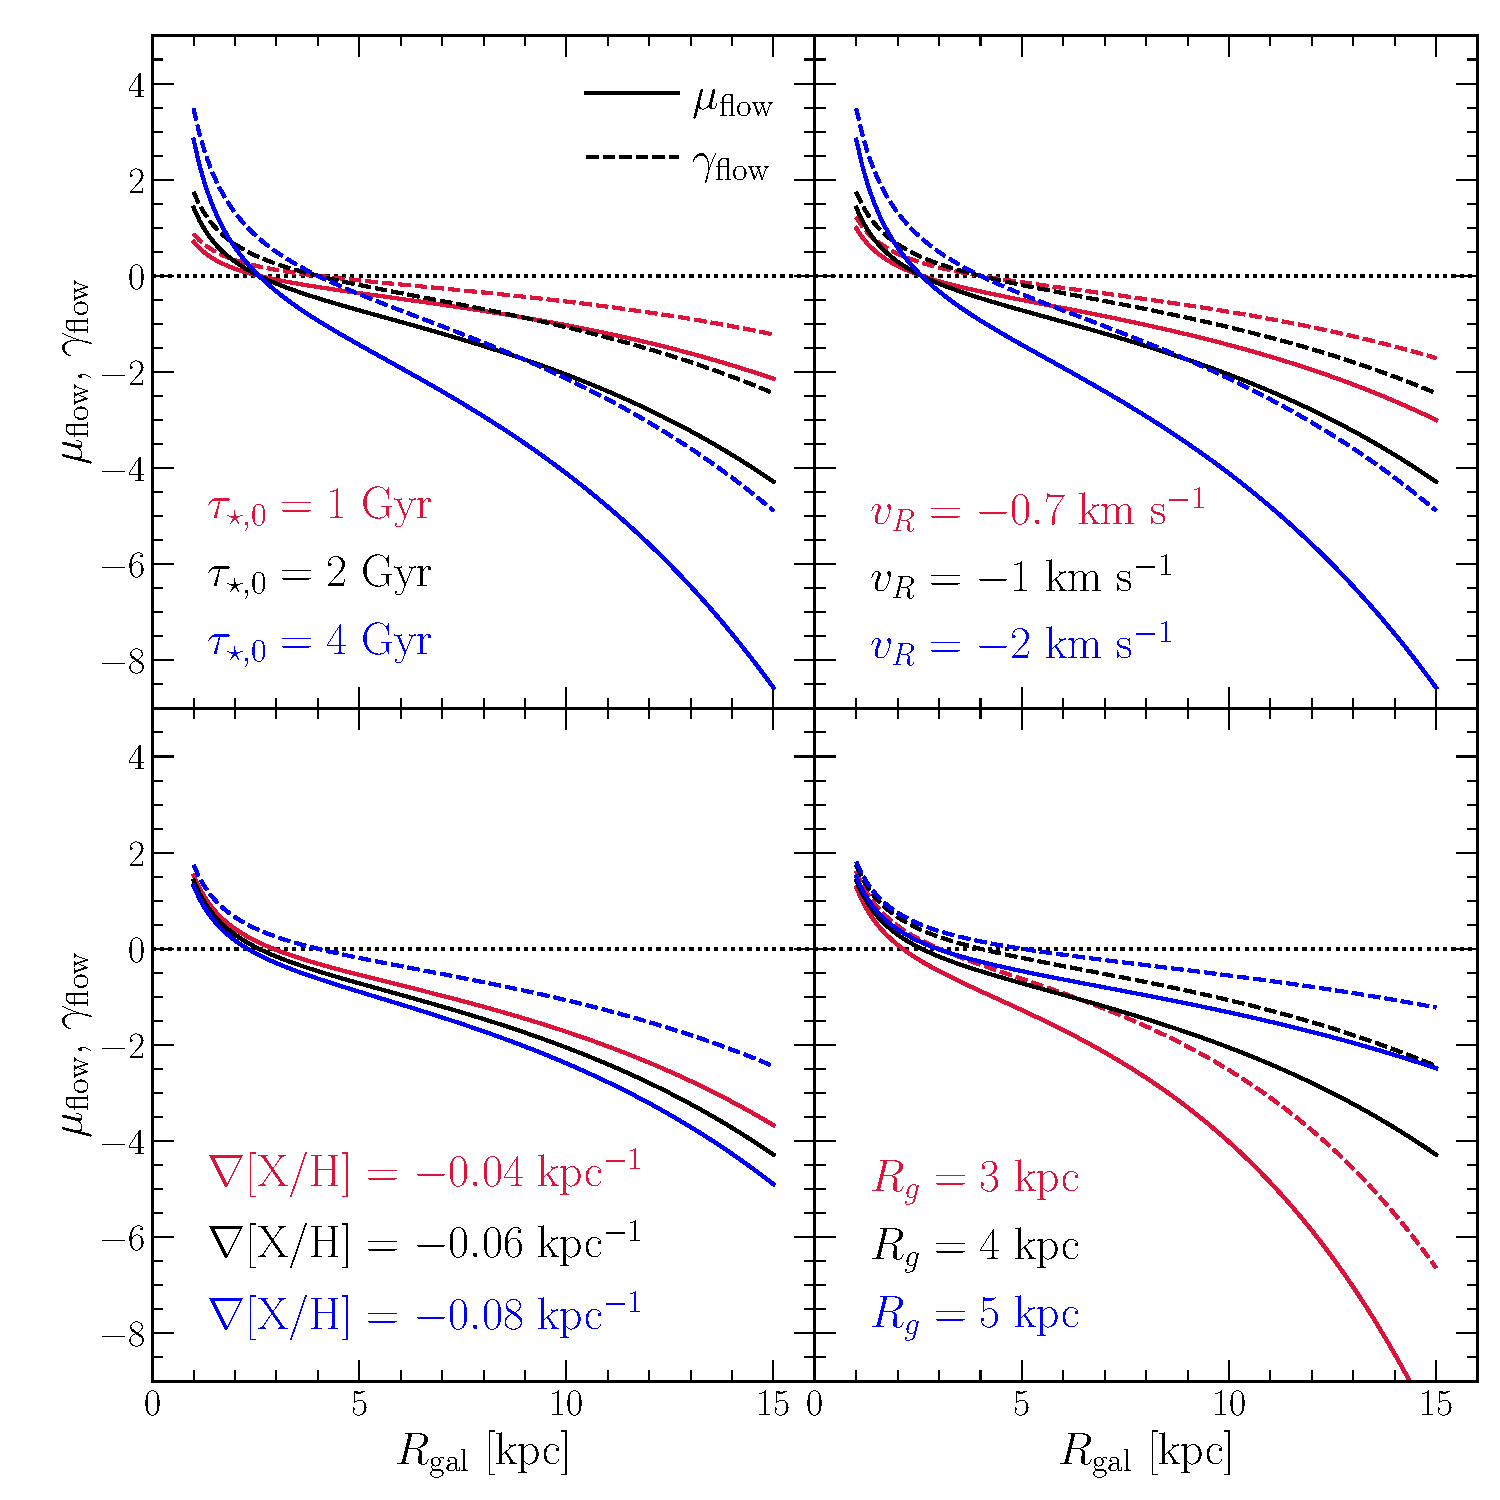
\includegraphics[scale = 0.5]{chapter7/muflow_gammaflow_vs_radius.pdf}
\caption{
The radial flow coefficients~$\mu_\flow$ (solid) and~$\gamma_\flow$ (dashed) as
functions of radius for different parameter choices.
Black lines correspond to the fiducial choice of
($\tau_{\star,0}$,~$v_R$,~\grad{X},~$R_g$) = (2 Gyr, 1 km s$^{-1}$,
$-0.06$ kpc$^{-1}$,~$4$ kpc) and are the same in all panels.
Each panel then shows variations in one of these four parameters according to
the legends in the lower right.
We also mark~$\mu_\flow$,~$\gamma_\flow = 0$ with a black dashed line, marking
the boundary between a radial flow acting as a source versus a sink of metals
and gas, respectively.
}
\label{outflows:fig:flow-coefficients-vs-radius}
\end{figure*}

Fig.~\ref{outflows:fig:flow-coefficients-vs-radius} shows~$\mu_\flow$
and~$\gamma_\flow$ as a function of radius for different parameter choices.
By definition, radial flows are a~\textit{source} of metals when~$\mu_\flow > 0$
and a~\textit{sink} when~$\mu_\flow < 0$; the same is true of the gas supply
with~$\gamma_\flow$.
In general, radial flows are a sink of both gas and metals across most of the
Galactic disk, becoming a source term only at radii better associated with the
bulge.
We expect this result to be generic as the negative sign arises due to the
difference between~$1 / R$, which varies, and~$1 / R_g + 1 / R_x$, which is
constant for a given parameter selection.
Flows are however a stronger sink for metals than gas under this
parameterization since, by definition,~$\mu_\flow = \gamma_\flow + \tau_\star
v_R / R_x$ and~$v_r < 0$.
Both~$\tau_{\star,0}$ and~$v_R$ are normalizing factors on the flow
coefficients, so they do not impact the radius at which~$\mu_\flow = 0$ or
$\gamma_\flow = 0$, but increases in their values make flows a stronger sink
where they are a sink and a stronger source where they are a source.
Changes in the slopes of gradients, either metallicity or gas surface density,
impact the flow rates in an intuitive manner: they are a stronger sink for more
sharply declining gradients as the mass or metallicity at~$R + \Delta R$ is
smaller in these cases.
Interestingly, the exact slope of the metallicity gradient~\grad{X} has minimal
impact on~$\mu_\flow$, potentially indicating that radial flows in turn have
minimal impact on abundance gradients.




% In Appendix~\ref{outflows:sec:coefficients-derivation}, we demonstrate that the
% effects of radial flows in a Milky Way-like disk can be understood with the
% coefficients~$\gamma_\flow$ and~$\mu_\flow$
% \begin{subequations}\begin{align}
% \gamma_\flow &= -\tau_\star v_R
% \left(\frac{1}{R} - \frac{1}{R_g}\right)
% \label{outflows:eq:gamma-flow}
% \\
% \mu_\flow &= -\tau_\star v_R
% \left(\frac{1}{R} - \frac{1}{R_g} - \frac{1}{R_x}\right),
% \label{outflows:eq:mu-flow}
% \end{align}\end{subequations}
% where~$R$ denotes Galactocentric radius,~$R_g$ is the scale radius of an
% exponential surface density gas disk, and~$R_x = -(\grad{X}~\ln 10)^{-1}$ is the
% scale radius of the metallicity gradient in~$Z_x$ implied by a linear gradient
% in [X/H].
% Because~$v_R < 0$ for inward radial flows, the length scale~$-\tau_\star v_R$
% is positive.
% \par
% The flow rates themselves and their impact on equations
% \refp{outflows:eq:mdot-gas} and~\refp{outflows:eq:mdot-element} are then given
% by
% \begin{subequations}\begin{align}
% \begin{split}
% \dot{M}_{g,\flow} &= \dot{M}_\star \gamma_\flow
% \\
% \implies \dot{M}_g &= \dot{M}_\text{in} - \dot{M}_\star
% \left(1 + \eta - \gamma_\flow - r\right)
% \end{split}
% \label{outflows:eq:mdot-gas-flow}
% \\
% \begin{split}
% \dot{M}_{x,\flow} &= Z_x \dot{M}_\star \mu_\flow
% \\
% \implies \dot{M}_x &= \ycc{$x$} \dot{M}_\star +
% \yia{$x$} \langle \dot{M}_\star \rangle_\text{Ia} -
% Z_x \dot{M}_\star \left(1 + \eta - \mu_\flow - r\right).
% \end{split}
% \label{outflows:eq:mdot-element-flow}
% \end{align}\end{subequations}






% 	\item Assuming infalling gas to be zero metallicity, the rate of a change
% 	of the mass of some element~$x$ in the ISM is given by
% 	\begin{equation}
% 	\dot{M}_x = \sum_i \dot{M}_{x,i} - Z_x \dot{M}_\star
% 	\left(1 + \eta - r\right),
% 	\end{equation}
% 	where~$Z_x = M_x / M_g$ is the mass fraction of~$x$ in the ISM
% 	and~$\sum_i \dot{M}_{x,i}$ generically accounts for enrichment channels
% 	such as core collapse supernovae (CCSNe), Type Ia supernovae (SNe Ia),
% 	asymptotic giant branch (AGB) stars, etc. which may produce~$x$ in some
% 	significant amount.
% 	In the case of O and Mg, there are arguments from both theoretical
% 	\citep[e.g.,][]{Andrews2017, Limongi2018} and empirical
% 	\citep{Griffith2019, Griffith2022, Weinberg2019, Weinberg2022}
% 	perspectives suggesting that their population-averaged yields are dominated
% 	by massive stars with a metallicity-independent yield.
% 	In this case, the above expression reduces to
% 	\begin{equation}
% 	\dot{M}_x \approx \ycc{$x$} \dot{M}_\star - Z_x \dot{M}_\star
% 	\left(1 + \eta - r\right),
% 	\end{equation}
% 	where~$\ycc{$x$}$ is the yield of~$x$.
% 	This expression retains the approximations from {\color{red} previous
% 	chapters} that enrichment from CCSNe occurs instantaneously after a single
% 	stellar population's formation, which is valid as long as the timescales of
% 	galaxy evolution are much longer than the lifetimes of massive stars.

% 	\item \citet{Weinberg2017b} demonstrate that the first-order details of the
% 	enrichment history in the ISM are determined by~$\eta$ and the star
% 	formation efficiency timescale~$\tau_\star \equiv M_g / \dot{M}_\star$.
% 	In the absence of sudden events such as bursts in star formation
% 	\citep[e.g.,][]{Johnson2020}, the detailed form of the SFH has minimal
% 	impact on the shape of the evolutionary track through chemical space
% 	(e.g., the~\afe-\feh~plane), with that information instead encoded in the
% 	density of stars along the track.
% 	However, in the absence of outflows (i.e.,~$\eta = 0$), then the shape of
% 	the SFH has a stronger effect, and radial flows have a stronger effect.
% 	{\color{red} Some short discussion on why~$\eta = 0$ versus~$\eta \neq 0$
% 	is interesting, potentially just referencing the discussion in the
% 	introduction}.

% 	\item {\color{red} Speaking of radial flows and Segways!}
% 	Under the approximation that all of the gas in some ring flows
% 	inward or outward with a single velocity~$v_R$, we demonstrate in
% 	Appendix~\ref{outflows:sec:coefficients-derivation} that the rate of change
% 	of the mass of some element~$x$ due solely to this process can be expressed
% 	as
% 	\begin{equation}
% 	\dot{M}_{x,\flow} = Z_x \dot{M}_\star \mu_\flow,
% 	\end{equation}
% 	where~$\mu_\flow$ is a unitless coefficient given by
% 	\begin{equation}
% 	\mu_\flow \equiv -\tau_\star v_R
% 	\left(\frac{1}{R} - \frac{1}{R_g} - \frac{1}{R_x}\right).
% 	\end{equation}
% 	$R_g$ is the scale radius of the gas disk, and~$R_x \equiv
% 	-(\grad{X} \ln 10)^{-1}$ is the scale radius of the exponential gradient
% 	in~$Z_x$ implied by a linear gradient in [X/H].

% 	\item Similarly, the rate of change of the ISM mass due to radial flows is
% 	given by
% 	\begin{equation}
% 	\dot{M}_{g,\flow} = \dot{M}_\star \gamma_\flow,
% 	\end{equation}
% 	where~$\gamma_\flow$ is given by
% 	\begin{equation}
% 	\gamma_\flow \equiv -\tau_\star v_R
% 	\left(\frac{1}{R} - \frac{1}{R_g}\right)
% 	= \mu_\flow - \frac{\tau_\star v_R}{R_x}.
% 	\end{equation}

% 	\item The coefficients~$\mu_\flow$ and~$\gamma_\flow$ have an explicit
% 	$1 / R$ dependence on radius, though in principle variations in the SFE
% 	timescale~$\tau_\star$ should also shape their variations with radius.
% 	A simple parameterization of~$\tau_\star$ with radius can be motivated by
% 	combining the Kennicutt-Schmidt scaling~\citep[e.g.,][]{Schmidt1959,
% 	Schmidt1963, Kennicutt1998} with its definition:
% 	\begin{equation}\begin{split}
% 	\tau_\star &\equiv \frac{M_g}{\dot{M}_\star}
% 	= \frac{\Sigma_g}{\dot{\Sigma}_\star}
% 	\\
% 	&\propto \frac{\Sigma_g}{\Sigma_g^N}
% 	\\
% 	&= \tau_{\star,0} e^{(N - 1) R / R_g},
% 	\end{split}\end{equation}
% 	where~$\tau_{\star,0}$ is a normalizing constant setting the value of
% 	$\tau_\star$ at~$R = 0$.
% 	In short, the decrease in surface density of gas should in principle imply
% 	an increase in~$\tau_\star$ with increasing radius.
% 	If~$N = 1.5$, consistent with~\citet{Kennicutt1998}, then~$\tau_\star$
% 	increases exponentially with a scale radius exactly twice that of the gas
% 	disk itself.
% 	Based on the presence of the central molecular zone in the Milky Way
% 	\citep[e.g.,][]{Morris1996, Dahmen1998, PiercePrice2000, Hatchfield2020}
% 	and~\citeauthor{Leroy2008}'s~\citeyearpar{Leroy2008} measurement of
% 	$\tau_\star = 2$ Gyr for molecular gas, we adopt~$\tau_{\star,0} = 2$ Gyr
% 	as a fiducial value.

% \end{itemize}

% \begin{itemize}

% 	\item $\mu_\flow$ and~$\gamma_\flow$ are parameterized such that radial
% 	flows are a source if they are positive and a sink if they are negative.
% 	For an inward gas flow (i.e.,~$v_R < 0$),~$\gamma_\flow > \mu_\flow$.

% 	\item $0 \leq \gamma_\flow \leq -\tau_\star v_R / R_x$ is an interesting
% 	region of parameter space in that radial flows are a~\textit{source} of
% 	gas ($\gamma_\flow > 0$) but a~\textit{sink} of metals ($\mu_\flow < 0$).
% 	Dilution can be a strong effect in this scenario.

	% \item To understand the impact of radial flows on the metallicity gradient,
	% we must incorporate the effects on both metal and gas masses separately as
	% the metals are affected by the gradient but the gas is not.
	% Isolating the terms~$\dot{M}_{x,\flow}$ and~$\dot{M}_{g,\flow}$:
	% \begin{equation}\begin{split}
	% \dot{Z}_{x,\flow} &= \frac{\dot{M}_x M_g - M_x \dot{M}_g}{M_g^2}
	% \\
	% &= \frac{\dot{M}_x}{M_g} - \left(\frac{M_x}{M_g}\right)
	% \frac{\dot{M}_g}{M_g}
	% \\
	% \dot{Z}_{x,\flow} < 0 \implies \frac{\dot{M}_x}{M_g} &< Z_x
	% \frac{\dot{M}_g}{M_g}
	% \\
	% \frac{\dot{M}_x}{\dot{M}_g} &< Z_x
	% \\
	% \frac{Z_x \dot{M}_\star \mu_\flow}{\dot{M}_\star \gamma_\flow} &< Z_x
	% \\
	% \mu_\flow &< \gamma_\flow.
	% \end{split}\end{equation}


% \end{itemize}


